\section{Methoden}
	
	Dieser Abschnitt befasst sich mit dem Aufbau des Franck-Hertz-Versuches, so wie auch den dabei auftretenden Unsicherheiten.
	
	\subsection{Aufbau}		
		\begin{figure}[ht]
			\centering
			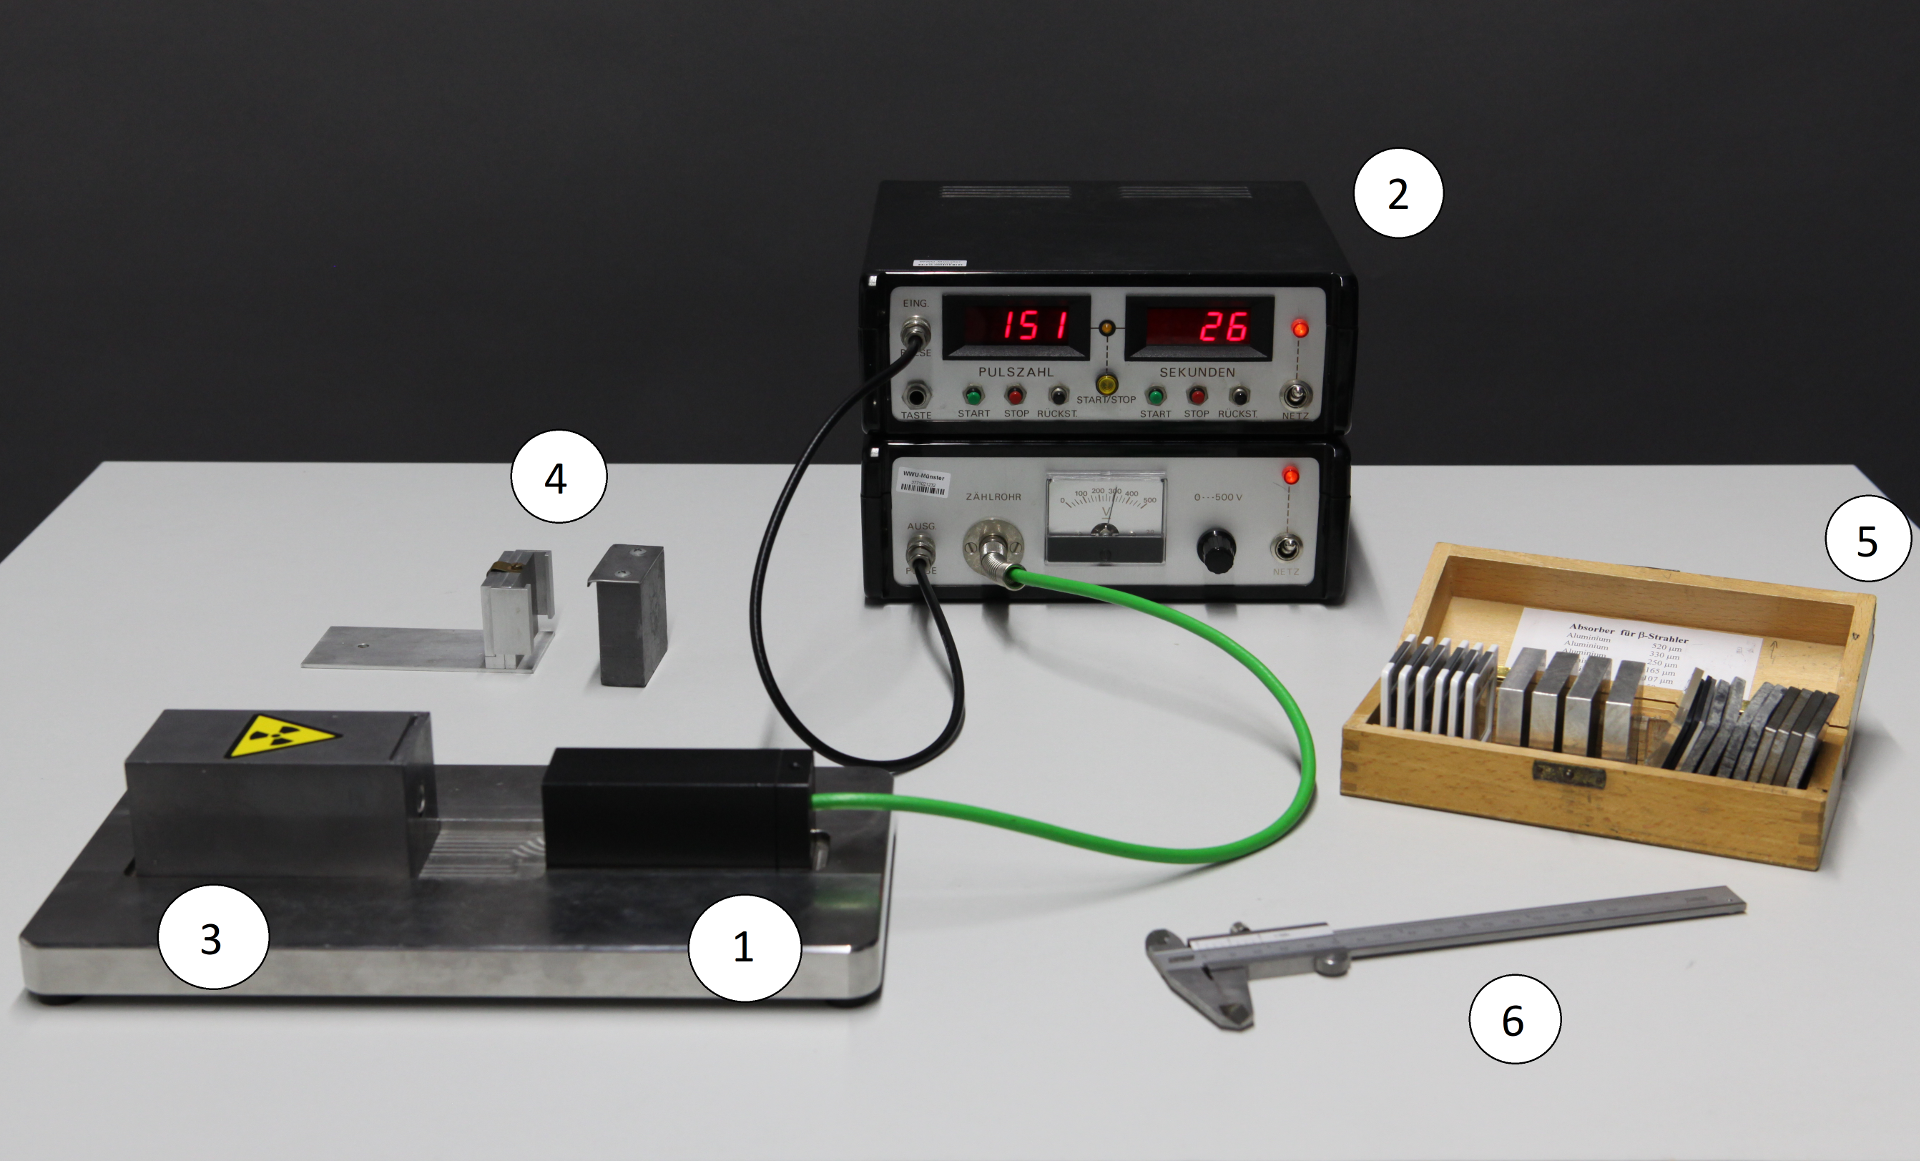
\includegraphics[width=\textwidth]{bilder/Aufbau.png}
			\caption{Diese Abbildung stellt die Schaltung der Franck-Hertz-Röhren (Hg links, Ne rechts) dar. \cite{WWU}}
			\label{fig:Aufbau}	
		\end{figure}	
		Wie in Abbildung \ref{fig:Aufbau} dargestellt, besteht der Aufbau des Franck-Hertz-Versuches im Wesentlichen aus einer Triode, welche mit einem Neongas bzw. flüssigem Quecksilber gefüllt ist. 
		Aus der Kathode werden Elektronen gelöst und zur Anode geschickt.
		Vor dem Gitter, welches zwischen Kathode und Anode liegt, werden diese mit der Beschleunigungsspannung	$U_B$ beschleunigt und hinter dem Gitter mit der Gegenspannung $U_G$ abgebremst.
		Bei der Neonröhre ist hinter der Kathode zusätzlich ein Steuergitter, um mit der Spannung $U_S$ die Raumladung in Kathodennähe zu verringern, sodass der Elektronenaustritt nicht verhindert wird.
		
		Da der elektrische Strom an der Anode sehr gering ist, wird stattdessen die dazu proportionale anliegende Spannung gemessen.
		Diese wird über Operationsverstärker im Betriebsgerät verstärkt und ist einfacher zu messen.
		  
		Für das Quecksilber werden zwei Messungen durchgeführt.
		Zum einen bei Zimmertemperatur, wo sich das Quecksilber größtenteils im flüssigem Zustand befindet, zum anderen bei deutlich erhöhter Temperatur, wo der Dampfdruck höher ist.
		Um das Quecksilber zu erhitzen, befindet sich die Quecksilberröhre in einem Ofen, der auf ca. $\SI{200}{\celsius}$ erhitzt wird
		Ein hoher Druck ist notwendig um eine Reihe von Elektronenstößen an den Atomen zu ermöglichen, welche die zu messende Charakteristiken ausmachen.
		
	\subsection{Unsicherheiten}
	
		Jegliche Unsicherheiten werden nach GUM bestimmt und berechnet\footnote{Die Gleichungen dazu finden sich im Anhang unter \ref{fig:GUM_combine}, \ref{fig:GUM_formula}.}.
		Für digitale Messungen wird eine Unsicherheit von $u(X) = \frac{\Delta X}{\sqrt{3}}$, bei analogen Messungen eine von $u(X) = \frac{\Delta X}{\sqrt{6}}$ angenommen.
	
		Bei diesem Versuch treten die Unsicherheiten primär bei den Digitalanzeigen der Messgeräte für Spannung und Temperatur auf.
		
		Die Beschleunigungsspannung wird analog eingestellt und mit einem digitalen Multimeter gemessen ($\Delta U = \SI{0.01}{\volt}$).
	
		Der Anodenstrom ist proportional zu der am Ausgang des Betriebsgerätes anliegenden Spannung.
		Diese wird ebenfalls mit einem digitalen Multimeter gemessen ($\Delta U = \SI{0.1}{\volt}, \SI{1}{\volt}$).
		Dabei ist der benutzte Wertebereich in der Messung berücksichtigt.
		
		Die Temperatur im Ofen wurde mit Hilfe eines digitalen Thermometers gemessen.
		Da die Temperatur im Ofen Schwankungen unterlag, wird die Unsicherheit etwas größer gewählt ($\Delta T = \SI{5}{\kelvin}$).
		
		Die Minima und Maxima der Beschleunigungsspannung wurden aus den Daten gelesen und dementsprechend bewertet ($\Delta U = \SI{0.5}{\volt}$) .
		
		Die Unsicherheiten von Konstanten und stoffspezifischen Eigenschaften, sowie dessen Quelle werden bei Bedarf angegeben.

\section{Durchführung und Datenanalyse}
	
	Vor der Aufnahme der Messungen wurde der Aufbau an ein Oszilloskop angeschlossen, um den Verlauf der Franck-Hertz-Kurven zu verbildlichen (siehe Abb. \ref{fig:kurveNe} und Folgende im Anhang).
	Für eine optimale Aufnahme der $I_A/U_B$-Charakteristiken wurde mit Hilfe des Oszilloskop die Gegenspannung $U_G$ gesucht, bei der die Charakteristiken am deutlichsten erkennbar waren.
	Diese Gegenspannung lag bei $ U_\text{G} \approx \SI{1}{\volt}$.
	
	Während der Aufnahme der Werte war bei der Neonröhre ein rötliches Leuchten zu erkennen, welches mit steigender Beschleunigungsspannung $U_B$ intensiver wurde. 
	Dies ist auf Elektronenstöße zurückzuführen.
	Je nachdem wie viel Energie ein Elektron besitzt, führt es (in)elastische Stöße mit den Atomen des Gases aus. 
	Hat es genug Energie um das Atom anzuregen, so gibt es diese an das Atom ab.
	Nachdem das Atom angeregt wurde, fällt es schnell in seinen Grundzustand zurück und emittiert dabei Licht mit entsprechender Wellenlänge.
	Die wahrscheinlichsten dieser Übergänge führen bei Neon zu einer Emission von rötlichem Licht 
	Bei dem Quecksilber war bei den beiden Messungen keine solche Beobachtung möglich.
	
	\begin{figure}[ht]
		\centering
		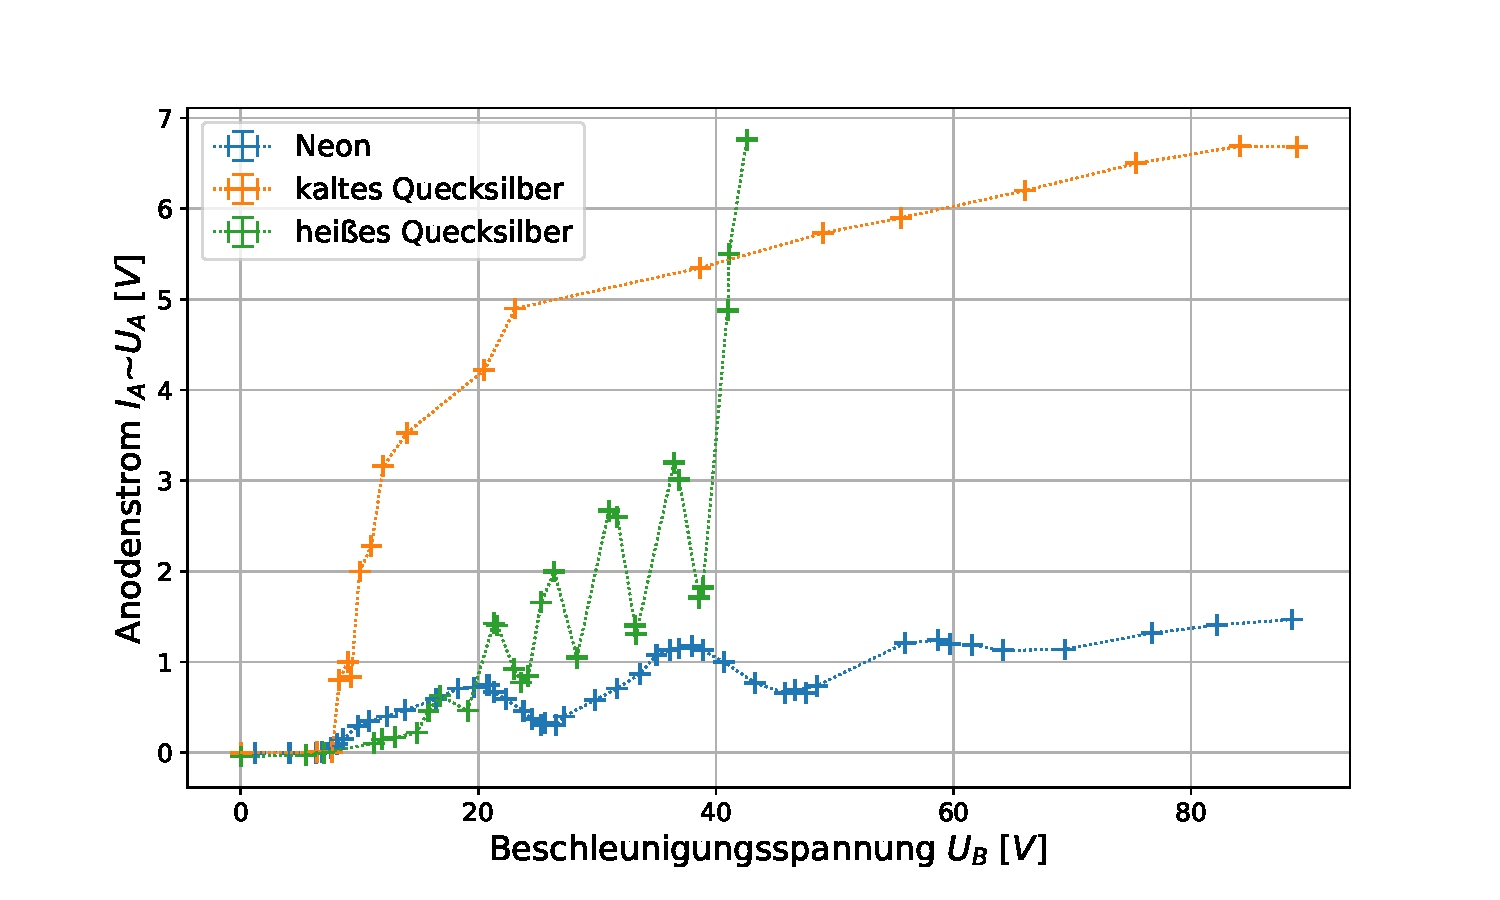
\includegraphics[width=\textwidth]{data/CharakteristikZusammen.pdf}
		\caption{$I_A/U_B$-Charakteristiken der Franck-Hertz-Röhren\footnote{Darstellung mit der Python-Bibliothek 'matplotlib'.}.}
		\label{fig:Kurve}	
	\end{figure}
	Die aufgenommen Werte für die $I_A/U_B$-Charakteristiken sind in Abbildung \ref{fig:Kurve} dargestellt\footnote{Um den Verlauf zwischen einzelnen Maxima und Minima zu skizzieren, sind die Messpunkte leicht miteinander verbunden. Der Verlauf wurde im Experiment bestätigt. Da für die Messung allerdings nur der Abstand der Maxima und Minima von Bedeutung sind, wurden die Zwischenräume weitgehend übersprungen.}. 
	Zu erkennen ist bereits, dass der Kurvenverlauf bei dem flüssigem Quecksilber der Kennlinie einen logarithmischen Verlauf annimmt, wohingegen bei dem Neon und noch ausgeprägter bei dem erhitzten Quecksilber der gemessene Anodenstrom wiederholt zu- und abnimmt, so dass ein "zackiges" Muster entsteht.\footnote{Die Linien zwischen den Messwerten dienen nur zur Verbildlichung und entsprechen nur genähert dem beobachteten Spannungsverlauf. Bei den Geraden handelt es sich eigentlich um  Kurven mit hoher Steigung (bzw. hohem Abfall)}. 
	Bei dem heißen Quecksilber sind fünf Maxima erkennbar, bei dem Neon hingegen drei.
	Dies zeigt, dass die Restenergie der Elektronen nach dem Stoß nicht ausreicht, um die Gegenspannung zu überwinden, weswegen der Anodenstrom geringer wird.
	Erhöht man die Beschleunigungsspannung weiter, so steigt der Anodenstrom erneut, fällt jedoch wieder ab sobald die Elektronen genug Energie besitzen um zwei Atome anzuregen.
	Dadurch ergibt sich der charakteristische Verlauf der Franck-Hertz-Kurve.
	Die Anregungsspannungen entsprechen den Werten für die Energien in \si{\electronvolt}.
	 
	Mit Hilfe dieser Messungen lassen sich über die Abstände der Minima bzw. Maxima (hier wurde der Mittelwert von beiden gebildet) die Energien der Elektronen bestimmen, die nötig sind um die Atome der Gase anzuregen.
	Dazu dient $E=eU$. 
	Die Wellenlänge des emittierten Lichts bestimmt sich über $\lambda = \frac{h \cdot c}{E}$.
	Dabei ist $h$ das planck'sche Wirkungsquantum.
	Ebenso lässt sich die Frequenz durch $f = \frac{c}{\lambda}$ ermitteln. 
	In Tabelle \ref{tab:Werte} sind die benötigten Energien für die Anregungen der Atome in den Gasen, sowie auch die Frequenzen und Wellenlängen des daraufhin emittierten Lichts, verzeichnet.
	\begin{table}
		\caption{In dieser Tabelle sind die ermittelten Energien, Wellenlängen und Frequenzen dargestellt\footnote{Unsicherheitsformeln zu den einzelnen Werten im Anhang unter .}%TODO Anhang Unsicherheitsrechnungen referenz
		\label{tab:Werte}
		\centering
		\begin{tabular}{c|c|c|c}
			& E & $\lambda$ & $f$ \\			
			\hline		
			Ne & \SI{19.23+-0.10}{\electronvolt} & \SI{64.49+-0.34}{\nano\meter} & \SI{4649+-25}{\tera\hertz} \\
			Hg(g) & \SI{4.90+-0.05}{\electronvolt} & \SI{253.0+-2.6}{\nano\meter} & \SI{1185+-12}{\tera\hertz} \\				
		\end{tabular}
	\end{table}

	Zur Bestimmung des Dampfdrucks in der Quecksilberröhre dient die Clausius-Clapeyron Formel (\ref{eq:Clausius}):
	\begin{align} \label{eq:Clausius}
		\ln(\frac{p_2}{p_1}) &= \frac{\Delta H_\text{m,v}}{R}\left( \frac{1}{T_2} - \frac{1}{T_1} \right) \\
		p_2 &= \exp{\frac{H_\text{m,v}}{R} \left( \frac{1}{T_2} - \frac{1}{T_1} \right) } \cdot p_1
	\end{align}
	Dabei dient der Siedepunkt von Quecksilber als Referenzpunkt\cite{boilingPoint}\footnote{Wie in der Quelle unter dem Punkt Conclusions angemerkt, kann den beiden Werten eine relative Unsicherheit von 1\% zugeordnet werden.}.
	Die Werte sind $T_1 = \SI{629.77}{K}$, sowie $p_1 = \SI{101.325}{\kilo\pascal}$.
	$R = \SI{8.3145}{\joule\per\mol\per\kelvin}$ ist die allgemeine Gaskonstante\cite{Constants} und $H_\text{m,v} = \SI{59.3+-0.1}{\kilo\joule\per\mol}$ die molare Verdampfungsenthalpie bzw. spezifische Verdampfungswärme\cite{verdampfungswaerme}.
	Die Gleichung lässt sich dann nach $p_2$ umstellen und mit den gemessenen Temperaturen $T_2 = \SI{291.15}{\kelvin}$, also Raumtemperatur bzw. $T_2 = \SI{465.15}{\kelvin}$ ausrechnen.
	Es folgen die Dampfdrücke $p_\text{kalt} = \SI{0.193+-0.035}{\pascal}$, also ein sehr starkes Vakuum, sowie $p_\text{warm} = \SI{1.84+-0.20}{\kilo\pascal}\approx \SI{0.02}{\bar}$, was immer noch ein sehr geringer Druck ist.
	
	Damit lässt sich nun die freie Weglänge der Elektronen in der Röhre berechnen.
	Dazu die Gleichung \ref{eq:Weg}:
	\begin{align} \label{eq:Weg}
		\lambda_\text{frei} = \frac{k_\text{B}\cdot T}{\sigma\cdot p}.
	\end{align}
 	Einsetzen mit $\sigma = \pi r_e^2$\cite{Constants} ergibt bei Raumtemperatur $\lambda_\text{frei, kalt} = \SI{8.4+-1.5}{10^8\meter}$ und erhitzt $\lambda_\text{frei, warm} = \SI{1.40+-0.15}{10^6\meter}$. 

\section{Diskussion}
	
	Die Ergebnisse dieses Versuches stützen weitgehend die Beschreibung der Gesetzmäßigkeiten bei Elektronenstößen an Atomen von J. Franck und G. Hertz.
	Es ließen sich bei dem Neon, wie auch bei dem erhitzten Quecksilber der charakteristische Verlauf der Franck-Hertz-Kurve erkennen.
	\begin{figure}[ht]
		\centering
		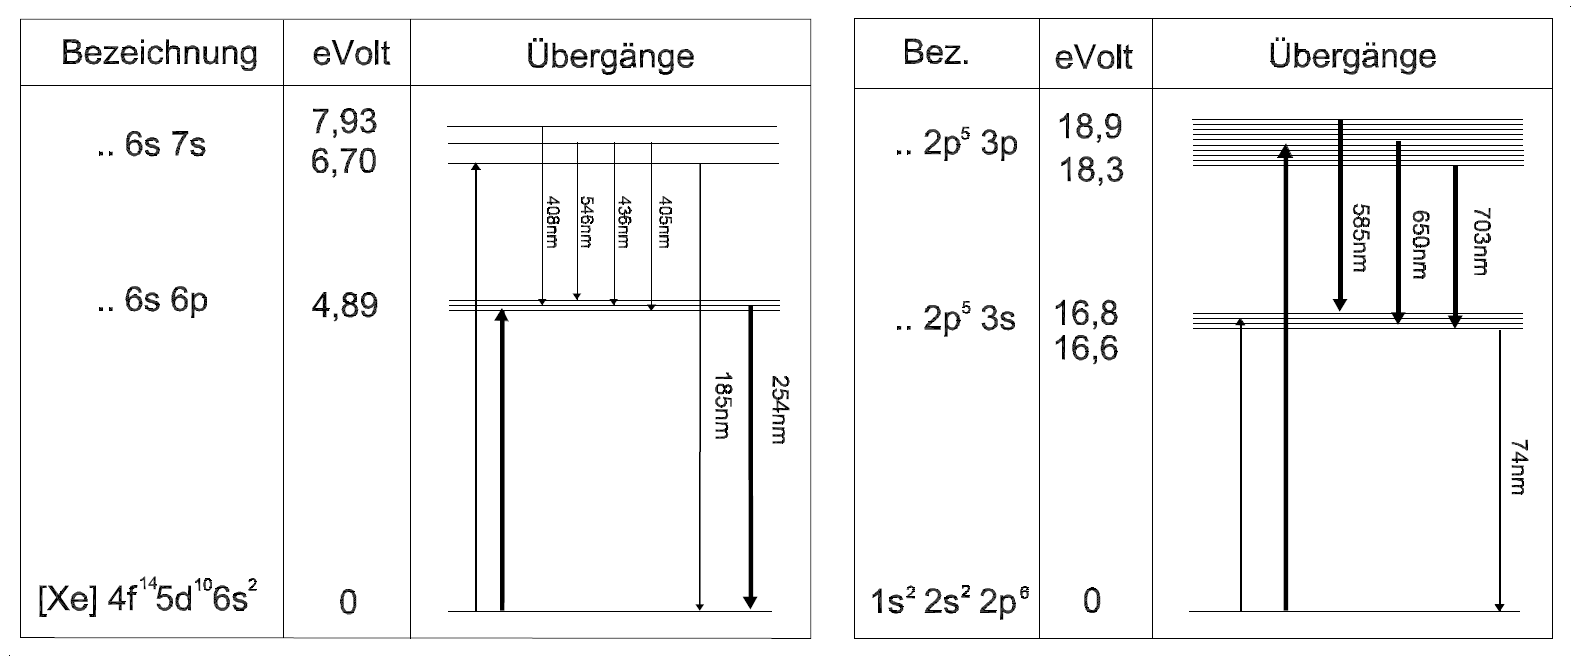
\includegraphics[width=\textwidth]{bilder/Uebergaenge.png}
		\caption{Diese Abbildung stellt das vereinfachte Termschemata von Quecksilber (links) und Neon (rechts) dar. Wahrscheinlichere Übergänge sind mit dickeren Pfeilen hervorgehoben.\cite{WWU}}
		\label{fig:Übergänge}	
	\end{figure}
	Auch die Energien, die durch diese Kurven berechnet wurden korrelieren mit den in Abbildung \ref{fig:Übergänge} dargestellten Literaturwerten der Energien für die Übergänge von Neon und Quecksilber. 
	Bei dem Quecksilber unterscheidet sich der berechnete Wert von \SI{4.90+-0.05}{\electronvolt} nur um 0,2\% von der ..6s6p-Übergangsenergie und die \SI{19.23+-0.10}{\electronvolt} von Neon nur um 1,7\% von der ..2p3p-Übergangsenergie.
	Diese Übergänge gehören zudem zu den häufiger auftretenden, was ebenfalls zu erwarten war.
	Vergleicht man nun die berechneten Wellenlängen, so unterscheidet sich die des Quecksilbers auch hier nur um 0,4\% von dem Literaturwert. 
	Bei dem Neon ist jedoch keine Wellenlänge des Lichts gegeben, welches bei dem Zurückfallen aus ..2p3p nach 1s2s2p entstehen würde. 
	Vergleicht man die berechneten \SI{64.49+-0.34}{\nano\meter} stattdessen mit den bei einem Sprung einer tieferen Schale zum Ruhezustand entstehenden  \SI{74}{\nano\meter}, so ist zu folgern, dass der Sprung aus einer höheren Schale Licht mit größerer Energie emittiert, was sinngemäß erscheint.
	
	Betrachtet man nun die Sichtbarkeit des emittierten Lichts, so lassen sich die Beobachtungen anhand der Abbildung \ref{fig:Übergänge} einfach erklären:
	Bei der Neonröhre war rötliches Licht zu sehen und häufige Übergänge führen zu emittiertem Licht mit Wellenlängen um \SI{600}{\nano\meter}, wo sich das rötliche Licht im sichtbaren Spektrum befindet.
	Bei dem Quecksilber ist es zwar möglich Licht im sichtbaren Bereich zu emittieren, welches violett oder bläulich scheinen würde, jedoch sind diese Übergänge deutlich seltener als solche im Ultraviolettbereich.
	
	Dass das Quecksilber bei Raumtemperatur die Charakteristiken der Franck-Hertz-Kurve nicht besitzt liegt daran, dass sich bei solch niedrigen Temperaturen kaum Quecksilberatome im gasförmigen Zustand befinden.
	Es kommt kaum zu Elektronenstößen und die Elektronen können beinahe ungehindert zur Kathode gelangen.
	Dadurch bildet sich stattdessen die für eine Triode typische charakteristische kurve aus, welche einen ungefähren logarithmischen Verlauf hat.
	
	Jedoch liegen die berechneten Werte der freien Weglänge deutlich über den erwarteten Werten.
	Die mittlere freie Weglänge bei Raumtemperatur ist größer als der Abstand zwischen Kathode und Gitter, was sich mit dem niedrigen Druck bei Raumtemperatur deckt.
	Während die Weglänge bei Ofentemperatur immerhin niedriger ist, als die bei Raumtemperatur, so ist sie immer noch viel größer als der Abstand Kathode-Gitter.
	
		